\documentclass[12pt]{ociamthesis}  % default square logo 
%\documentclass[12pt,beltcrest]{ociamthesis} % use old belt crest logo
%\documentclass[12pt,shieldcrest]{ociamthesis} % use older shield crest logo

%load any additional packages
\usepackage{amssymb}
\usepackage{multirow}
\usepackage{caption}
\usepackage{titlesec}
\usepackage{charter}
\usepackage{subfiles}
\usepackage{etoolbox}


\title{\large RESUME PYTHON}
\author{Jefrinanda Iaspartogi Marbun}             %your name
\college{1.18.4.052\\[5ex]} \\



%\renewcommand{\submittedtext}{change the default text here if needed}
\degree{Politeknik Pos Indonesia}     %the degree
\degreedate{Bandung}         %the degree date
\degreedate{2019}  

%end the preamble and start the document
\begin{document}

%this baselineskip gives sufficient line spacing for an examiner to easily
%markup the thesis with comments
\baselineskip=18pt plus1pt

%set the number of sectioning levels that get number and appear in the contents
\setcounter{secnumdepth}{3}
\setcounter{tocdepth}{3}


\maketitle                 


\chapter*{Chapter 2}
\section*{Jenis Variabel pada Python}
\par

 
Python memiliki seperangkat aturan pembuatan dan penulisan variabel yang jika dibandingkan dengan bahasa pemrograman lain seperti PHP, tidak jauh berbeda. Perlu diketahui bahwa Python merupakan bahasa pemrograman case sensitive. dan juga perlu diketahui nama variabel tidak boleh sama dengan salah satu nama yang masuk ke dalam kelompok {\textit{reserved word python}} , seperti : and, assert, break, class, continue, def, del, elif dsb. Variabel dalam python ada dua jenis yaitu variabel lokal dan global. berikut contoh variabel lokal dan global.

\begin{enumerate}
	\item buka Spyder lalu ketik kode berikut
	\begin{figure} [h]
	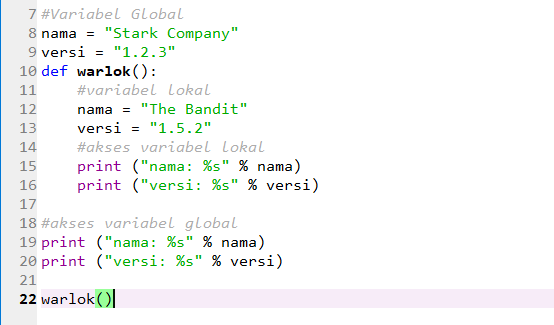
\includegraphics[width=9cm]{variabel/var1.png}
	\centering
	\end{figure}
	

	\item maka akan menghasilkan output seperti berikut
	\begin{figure} [h]
	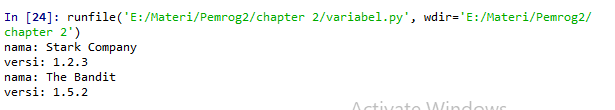
\includegraphics[width=12cm]{variabel/var2.png}
	\centering
	\end{figure}
	
	
\end{enumerate} 
\chapter*{ Input dari User}
\par
input dari user merupakan kodingan dimana user akan menuliskan dan akan ada output di layar. caranya sebagai berikut

\begin{enumerate}
	\item buka Spyder lalu ketik kode berikut
	\begin{figure} [h]
	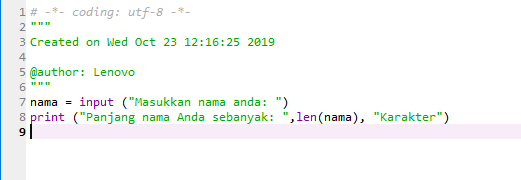
\includegraphics[width=9cm]{input/inp1.png}
	\centering
	\end{figure}
	

	\item maka akan menghasilkan output seperti berikut
	\begin{figure} [h]
	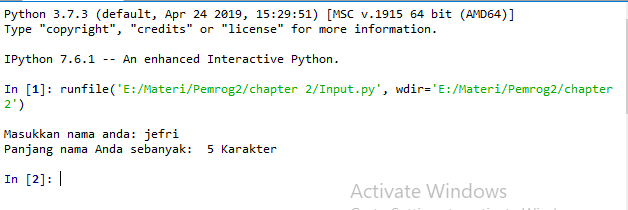
\includegraphics[width=9cm]{input/inp2.png}
	\centering
	\end{figure}
	
	
\end{enumerate}
\chapter*{Mengubah String ke Integer dan proses Aritmatika}

\par
didalam python tipe data dapat diubah dan dilakukan proses aritmatika didalamnya, contohnya sebagai berikut.

\begin{enumerate}
	\item buka spyder dan ketik kode sebagai berikut untuk mengubah dari string ke int.
	\begin{figure} [h]
	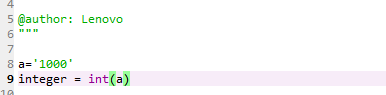
\includegraphics[width=12cm]{string/str1.png}
	\centering
	\end{figure}
	
	\item setelah itu maka ketika integer di print akan menghasilkan sebagai berikut
	\begin{figure} [h]
	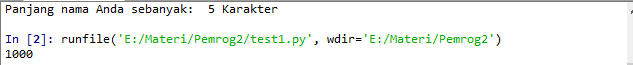
\includegraphics[width=12cm]{string/str2.png}
	\centering
	\end{figure}
	
	\item Setelah tipe data diubah, dapat langsung dikombinasikan dengan proses aritmatika
	
	\item untuk melakukan proses aritmatika maka dapat dilakukan dengan menuliskan kode sebagai berikut
	\begin{figure} [h]
	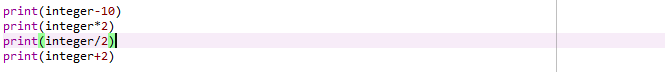
\includegraphics[width=12cm]{string/str3.png}
	\centering
	\end{figure}
	
	
	\item setelah menuliskan kode jangan lupa menuliskan perintah print
	
	\item setelah itu silahkan menjalankan script yang sudah dibuat
	

	
	

	\end{enumerate}
	
	


\section*{Perulangan}

\par
Didalam python, kita dapat melakukan proses perulangan. contohnya sebagai berikut.


\begin{enumerate}
	\item buka spyder lalu tulis script sebagai berikut.
	\begin{figure} [h]
	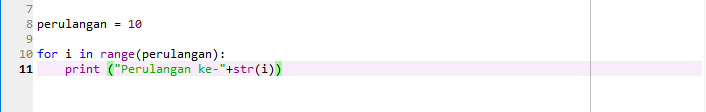
\includegraphics[width=9cm]{loop/loop1.png}
	\centering
	\end{figure}

\item kalian dapat mengisi jumlah loop yang akan dilakukan sesuai dengan keinginan kalian
	
    \item maka hasil ke layar akan menjadi sebagai berikut
	\begin{figure} [h]
	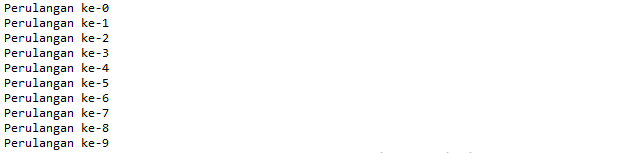
\includegraphics[width=9cm]{loop/loop2.png}
	\centering
	\end{figure}
	
	

\end{enumerate}
\section*{Cara pakai kondisi didalam kondisi}

\par
Didalam python kita dapat melakukan logika kondisi didalam kondisi. caranya sebagai berikut


 \begin{enumerate}
	\item buka aplikasi spyder lalu tuliskan codingan dengan logika dan kondisi sebagai berikut
	\begin{figure} [h]
	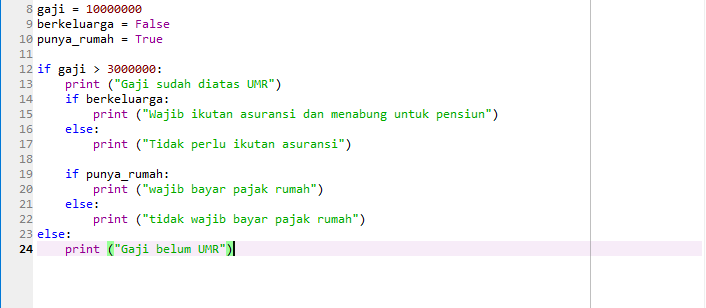
\includegraphics[width=9cm]{if/if1.png}
	\centering
	\end{figure}
	
	 
	\item kalian bisa memilih kondisi yang kalian inginkan. bisa False bisa True. dan mengisi jumlah gaji sesuai keinginan kalian
	
	\item Maka output akan seperti berikut
	\begin{figure} [h]
	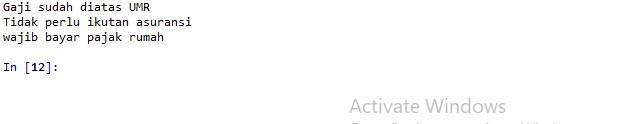
\includegraphics[width=10cm]{if/if2.png}
	\centering
	\end{figure}
	
	
	
	
	
    \end{enumerate}




\chapter*{Error yang biasa ditemukan saat melakukan sintak}
\section*{Error dalam menggunakan tanda kurung}
\begin{enumerate}
	\item dalam melakukan sintak print terkadang kita lupa untuk memberi tanda kurung sehingga sintak error
	\begin{figure} [h]
	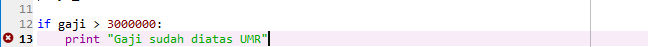
\includegraphics[width=12cm]{error/er1.png}
	\centering
	\end{figure}
	
    \item seharusnya ditulis seperti berikut
	\begin{figure} [h]
	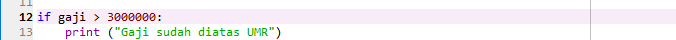
\includegraphics[width=12cm]{error/er2.png}
	\centering
	\end{figure}

\section*{Error penulisan huruf besar pada kondisi}
	
	
	\item Terkadang kita juga lupa untuk menggunakan huruf besar saat melakukan sintak kondisi 
	\begin{figure} [h]
	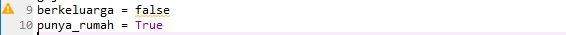
\includegraphics[width=9cm]{error/er3.png}
	\centering
	\end{figure}
	
	\item Seharusnya dituliskan sebagai berikut 
	\begin{figure} [h]
	
\includegraphics[width=9cm]{error/er4.png}
	\centering
	\end{figure}
	
	
\end{enumerate}
\chapter*{Try and Except}

\par
Didalam Python bisa melakukan sintak untuk Try and Except. Caranya sebagai berikut :


\begin{enumerate}

	\item ketikan kode seperti berikut
	\begin{figure} [h]
	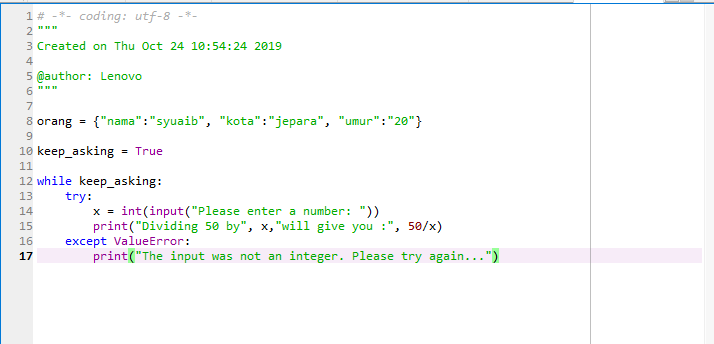
\includegraphics[width=12cm]{try/try1.png}
	\centering
	\end{figure}
	
	\item maka akan menghasilkan sebagai berikut
	\begin{figure} [h]
	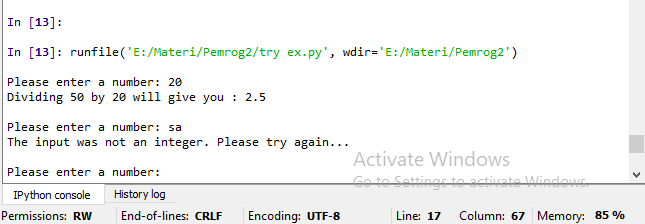
\includegraphics[width=12cm]{try/try2.png}
	\centering
	\end{figure}
	
	
	
	
\end{enumerate}

\chapter*{Perulangan "Apa Kabar" sejumlah 2 digit NPM }

\par
Kita bisa melakukan hal tersebut dengan inputan dari user yang membuat variabel, pengulangannya oleh batas range yang sudah diatur. Caranya sebagai berikut :


\begin{enumerate}
   

\item buka spyder dan ketikan kode seperti berikut
	\begin{figure} [h]
	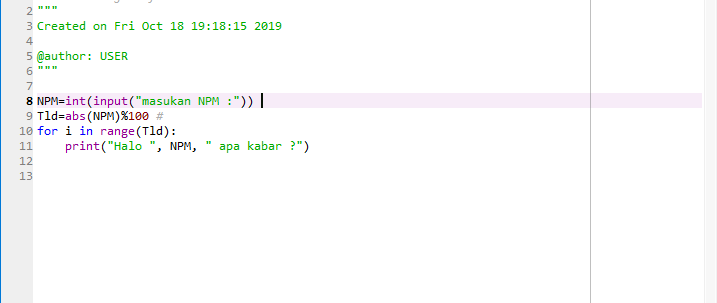
\includegraphics[width=10cm]{pakabs/pakabs.png}
	\centering
	\end{figure}
	
	
	
 \item maka akan tercetak 
 \begin{figure} [h]
	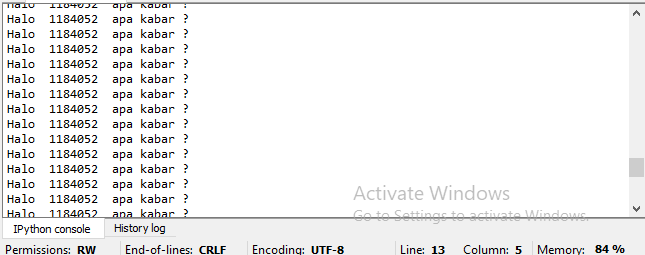
\includegraphics[width=9cm]{pakabs/pakabs2.png}
	\centering
	\end{figure}
 
	
	\end{enumerate}
\chapter*{Cara Print NPM }

\par
Kita bisa melakukan print NPM dengan nomor satu per satu caranya sebagai berikut.


\begin{enumerate}
   

\item buka spyder dan ketikan kode seperti berikut
	\begin{figure} [h]
	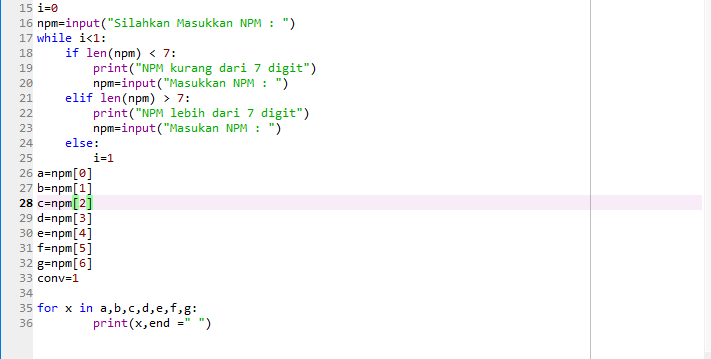
\includegraphics[width=10cm]{npm/npm3.png}
	\centering
	\end{figure}
	
	
	
 \item maka akan tercetak 
 \begin{figure} [h]
	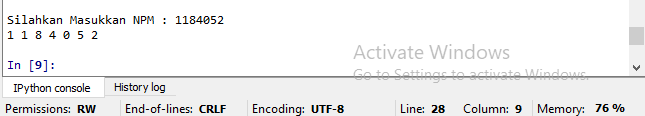
\includegraphics[width=9cm]{npm/npm4.png}
	\centering
	\end{figure}
 
	
	\end{enumerate}


\chapter*{Print NPM angka ganjil}
\par Kita juga dapat melakukan Print NPM yang hanya ganjil, dengan menggunakan logika modulus

\begin{enumerate}
   

\item buka spyder dan ketikan kode seperti berikut
	\begin{figure} [h]
	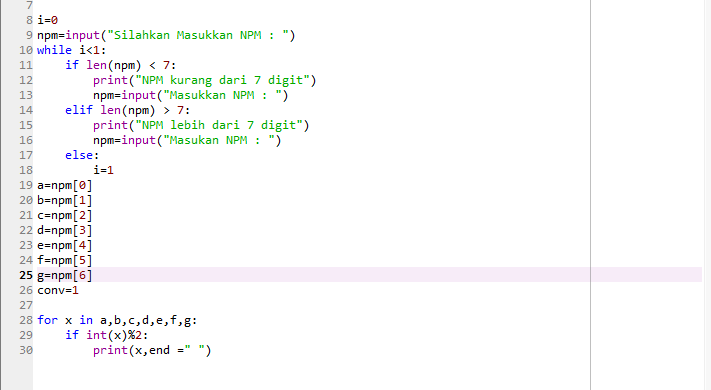
\includegraphics[width=7cm]{npm/npm1.png}
	\centering
	\end{figure}
	
	
	
 \item maka akan tercetak 
 \begin{figure} [h]
	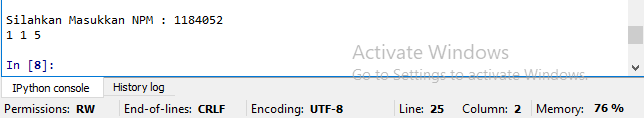
\includegraphics[width=7cm]{npm/npm2.png}
	\centering
	\end{figure}
 
	
	\end{enumerate}

\chapter*{Print NPM angka genap}
\par Kita juga dapat melakukan Print NPM yang hanya ganjil, dengan menggunakan logika modulus

\begin{enumerate}
   

\item buka spyder dan ketikan kode seperti berikut
	\begin{figure} [h]
	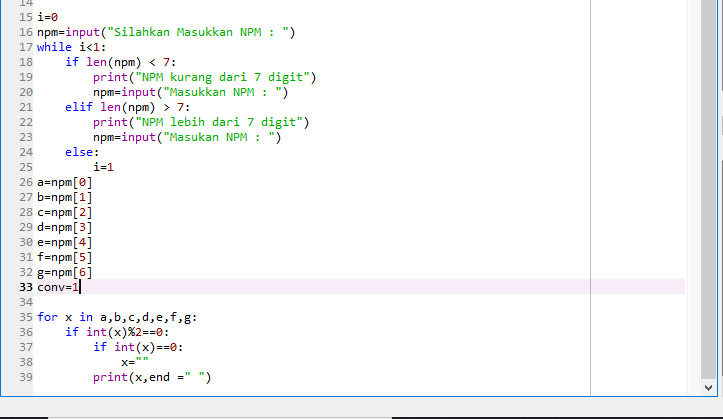
\includegraphics[width=7cm]{npm/npm5.png}
	\centering
	\end{figure}
	
	
	
 \item maka akan tercetak 
 \begin{figure} [h]
	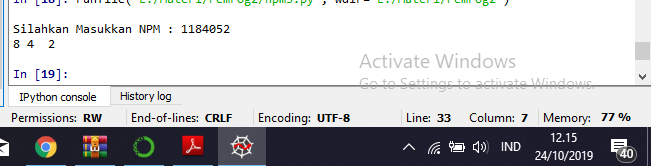
\includegraphics[width=7cm]{npm/npm6.png}
	\centering
	\end{figure}
 
	
	\end{enumerate}
\chapter*{Print NPM angka prima}
\par Kita juga dapat melakukan Print NPM yang hanya prima, dengan menggunakan logika modulus

\begin{enumerate}
   

\item buka spyder dan ketikan kode seperti berikut
	\begin{figure} [h]
	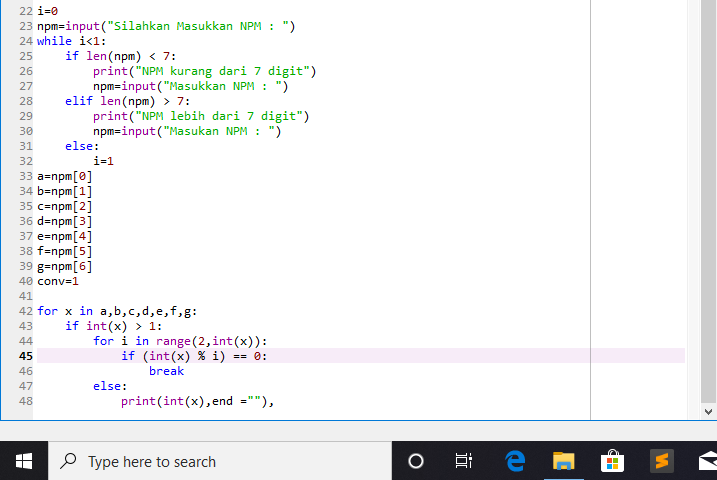
\includegraphics[width=7cm]{npm/npm7.png}
	\centering
	\end{figure}
	
	
	
 \item maka akan tercetak 
 \begin{figure} [h]
	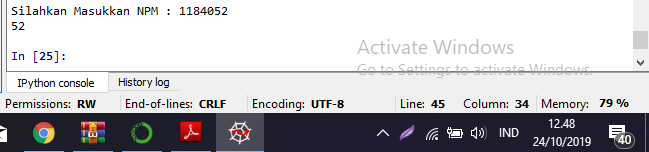
\includegraphics[width=7cm]{npm/npm8.png}
	\centering
	\end{figure}
 
	
	\end{enumerate}
\chapter*{Keterampilan Penanganan error}
\section*{peringatan error} 

\begin{enumerate}
   

\item ketik koding sebagai berikut
	\begin{figure} [h]
	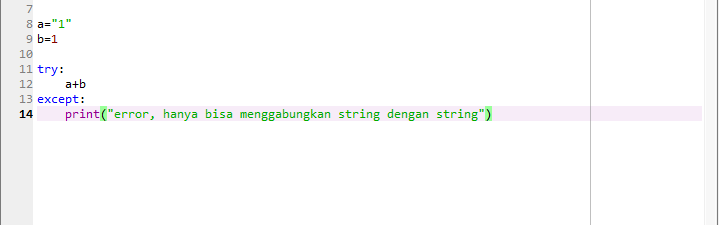
\includegraphics[width=7cm]{npm/npm10.png}
	\centering
	\end{figure}
	
	
	
 \item maka akan tercetak error sebagai berikut
 \begin{figure} [h]
	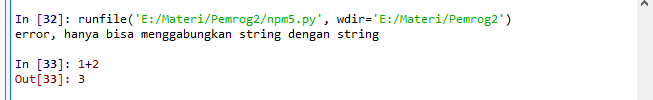
\includegraphics[width=7cm]{npm/npm11.png}
	\centering
	\end{figure}
 
	
	\end{enumerate}
\chapter*{Print NPM menggunakan pembagian npm dengan mod 3}
\par karna hasil bagi dengan mod 3 sama dengan 0 maka menggunakan bintang(*)
\begin{enumerate}
   

\item buka spyder dan ketikan kode seperti berikut
	\begin{figure} [h]
	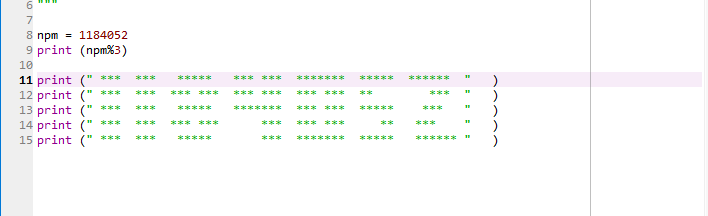
\includegraphics[width=7cm]{npm/npm13.png}
	\centering
	\end{figure}
	
	
	
 \item maka akan tercetak 
 \begin{figure} [h]
	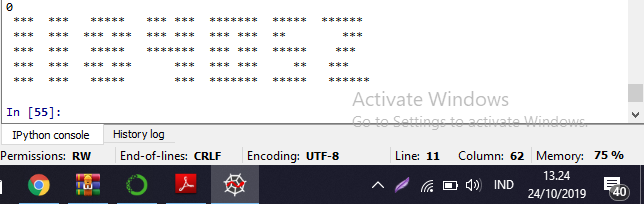
\includegraphics[width=7cm]{npm/npm14.png}
	\centering
	\end{figure}
 
	
	\end{enumerate}
\end{document}

